% Options for packages loaded elsewhere
\PassOptionsToPackage{unicode}{hyperref}
\PassOptionsToPackage{hyphens}{url}
\PassOptionsToPackage{dvipsnames,svgnames,x11names}{xcolor}
%
\documentclass[
  number]{elsarticle}

\usepackage{amsmath,amssymb}
\usepackage{lmodern}
\usepackage{iftex}
\ifPDFTeX
  \usepackage[T1]{fontenc}
  \usepackage[utf8]{inputenc}
  \usepackage{textcomp} % provide euro and other symbols
\else % if luatex or xetex
  \usepackage{unicode-math}
  \defaultfontfeatures{Scale=MatchLowercase}
  \defaultfontfeatures[\rmfamily]{Ligatures=TeX,Scale=1}
\fi
% Use upquote if available, for straight quotes in verbatim environments
\IfFileExists{upquote.sty}{\usepackage{upquote}}{}
\IfFileExists{microtype.sty}{% use microtype if available
  \usepackage[]{microtype}
  \UseMicrotypeSet[protrusion]{basicmath} % disable protrusion for tt fonts
}{}
\makeatletter
\@ifundefined{KOMAClassName}{% if non-KOMA class
  \IfFileExists{parskip.sty}{%
    \usepackage{parskip}
  }{% else
    \setlength{\parindent}{0pt}
    \setlength{\parskip}{6pt plus 2pt minus 1pt}}
}{% if KOMA class
  \KOMAoptions{parskip=half}}
\makeatother
\usepackage{xcolor}
\setlength{\emergencystretch}{3em} % prevent overfull lines
\setcounter{secnumdepth}{5}
% Make \paragraph and \subparagraph free-standing
\ifx\paragraph\undefined\else
  \let\oldparagraph\paragraph
  \renewcommand{\paragraph}[1]{\oldparagraph{#1}\mbox{}}
\fi
\ifx\subparagraph\undefined\else
  \let\oldsubparagraph\subparagraph
  \renewcommand{\subparagraph}[1]{\oldsubparagraph{#1}\mbox{}}
\fi


\providecommand{\tightlist}{%
  \setlength{\itemsep}{0pt}\setlength{\parskip}{0pt}}\usepackage{longtable,booktabs,array}
\usepackage{calc} % for calculating minipage widths
% Correct order of tables after \paragraph or \subparagraph
\usepackage{etoolbox}
\makeatletter
\patchcmd\longtable{\par}{\if@noskipsec\mbox{}\fi\par}{}{}
\makeatother
% Allow footnotes in longtable head/foot
\IfFileExists{footnotehyper.sty}{\usepackage{footnotehyper}}{\usepackage{footnote}}
\makesavenoteenv{longtable}
\usepackage{graphicx}
\makeatletter
\def\maxwidth{\ifdim\Gin@nat@width>\linewidth\linewidth\else\Gin@nat@width\fi}
\def\maxheight{\ifdim\Gin@nat@height>\textheight\textheight\else\Gin@nat@height\fi}
\makeatother
% Scale images if necessary, so that they will not overflow the page
% margins by default, and it is still possible to overwrite the defaults
% using explicit options in \includegraphics[width, height, ...]{}
\setkeys{Gin}{width=\maxwidth,height=\maxheight,keepaspectratio}
% Set default figure placement to htbp
\makeatletter
\def\fps@figure{htbp}
\makeatother
\newlength{\cslhangindent}
\setlength{\cslhangindent}{1.5em}
\newlength{\csllabelwidth}
\setlength{\csllabelwidth}{3em}
\newlength{\cslentryspacingunit} % times entry-spacing
\setlength{\cslentryspacingunit}{\parskip}
\newenvironment{CSLReferences}[2] % #1 hanging-ident, #2 entry spacing
 {% don't indent paragraphs
  \setlength{\parindent}{0pt}
  % turn on hanging indent if param 1 is 1
  \ifodd #1
  \let\oldpar\par
  \def\par{\hangindent=\cslhangindent\oldpar}
  \fi
  % set entry spacing
  \setlength{\parskip}{#2\cslentryspacingunit}
 }%
 {}
\usepackage{calc}
\newcommand{\CSLBlock}[1]{#1\hfill\break}
\newcommand{\CSLLeftMargin}[1]{\parbox[t]{\csllabelwidth}{#1}}
\newcommand{\CSLRightInline}[1]{\parbox[t]{\linewidth - \csllabelwidth}{#1}\break}
\newcommand{\CSLIndent}[1]{\hspace{\cslhangindent}#1}

\makeatletter
\makeatother
\makeatletter
\makeatother
\makeatletter
\@ifpackageloaded{caption}{}{\usepackage{caption}}
\AtBeginDocument{%
\ifdefined\contentsname
  \renewcommand*\contentsname{Table of contents}
\else
  \newcommand\contentsname{Table of contents}
\fi
\ifdefined\listfigurename
  \renewcommand*\listfigurename{List of Figures}
\else
  \newcommand\listfigurename{List of Figures}
\fi
\ifdefined\listtablename
  \renewcommand*\listtablename{List of Tables}
\else
  \newcommand\listtablename{List of Tables}
\fi
\ifdefined\figurename
  \renewcommand*\figurename{Figure}
\else
  \newcommand\figurename{Figure}
\fi
\ifdefined\tablename
  \renewcommand*\tablename{Table}
\else
  \newcommand\tablename{Table}
\fi
}
\@ifpackageloaded{float}{}{\usepackage{float}}
\floatstyle{ruled}
\@ifundefined{c@chapter}{\newfloat{codelisting}{h}{lop}}{\newfloat{codelisting}{h}{lop}[chapter]}
\floatname{codelisting}{Listing}
\newcommand*\listoflistings{\listof{codelisting}{List of Listings}}
\makeatother
\makeatletter
\@ifpackageloaded{caption}{}{\usepackage{caption}}
\@ifpackageloaded{subcaption}{}{\usepackage{subcaption}}
\makeatother
\makeatletter
\@ifpackageloaded{tcolorbox}{}{\usepackage[many]{tcolorbox}}
\makeatother
\makeatletter
\@ifundefined{shadecolor}{\definecolor{shadecolor}{rgb}{.97, .97, .97}}
\makeatother
\makeatletter
\makeatother
\ifLuaTeX
  \usepackage{selnolig}  % disable illegal ligatures
\fi
\usepackage[]{natbib}
\bibliographystyle{elsarticle-num}
\IfFileExists{bookmark.sty}{\usepackage{bookmark}}{\usepackage{hyperref}}
\IfFileExists{xurl.sty}{\usepackage{xurl}}{} % add URL line breaks if available
\urlstyle{same} % disable monospaced font for URLs
\hypersetup{
  pdftitle={Deconstructing Simple and Choice Decision and Movement Time Across the Spectrum of Schizophrenia Genetic Risk},
  pdfauthor={Joey Trampush3,2,; Samantha Fleck3; Dwight Dickinson2; Juan Pérez4; Max Mustermann},
  pdfkeywords={schizophrenia; reaction time; keyword 3},
  colorlinks=true,
  linkcolor={blue},
  filecolor={Maroon},
  citecolor={Blue},
  urlcolor={Blue},
  pdfcreator={LaTeX via pandoc}}

\setlength{\parindent}{6pt}
\begin{document}

\begin{frontmatter}
\title{Deconstructing Simple and Choice Decision and Movement Time
Across the Spectrum of Schizophrenia Genetic Risk}

\affiliation[1]{organization={true},,postcodesep={}}
\affiliation[2]{organization={true},,postcodesep={}}

\cortext[cor1]{Corresponding author}
        
\begin{abstract}
Text of abstract
\end{abstract}





\begin{keyword}
    schizophrenia; reaction time; keyword 3 \sep 
    schizophrenia; reaction time; keyword 3
\end{keyword}
\end{frontmatter}
    \ifdefined\Shaded\renewenvironment{Shaded}{\begin{tcolorbox}[breakable, enhanced, frame hidden, borderline west={3pt}{0pt}{shadecolor}, interior hidden, boxrule=0pt, sharp corners]}{\end{tcolorbox}}\fi

\textsuperscript{1} Keck School of Medicine of USC\\
\textsuperscript{2} National Institute of Mental Health\\
\textsuperscript{3} usc\\
\textsuperscript{4} Acme Corporation

\textsuperscript{*} Correspondence:
\href{mailto:joey.trampush@med.usc.edu}{Joey Trampush
\textless{}joey.trampush@med.usc.edu\textgreater{}}

Keywords: schizophrenia; reaction time; keyword 3

Highlights: These are the highlights.

\hypertarget{introduction}{%
\section{Introduction}\label{introduction}}

Here is a citation \citep{Marwick2017}

\hypertarget{background}{%
\section{Background}\label{background}}

\hypertarget{methods}{%
\section{Methods}\label{methods}}

\hypertarget{results}{%
\section{Results}\label{results}}

\begin{figure}

{\centering 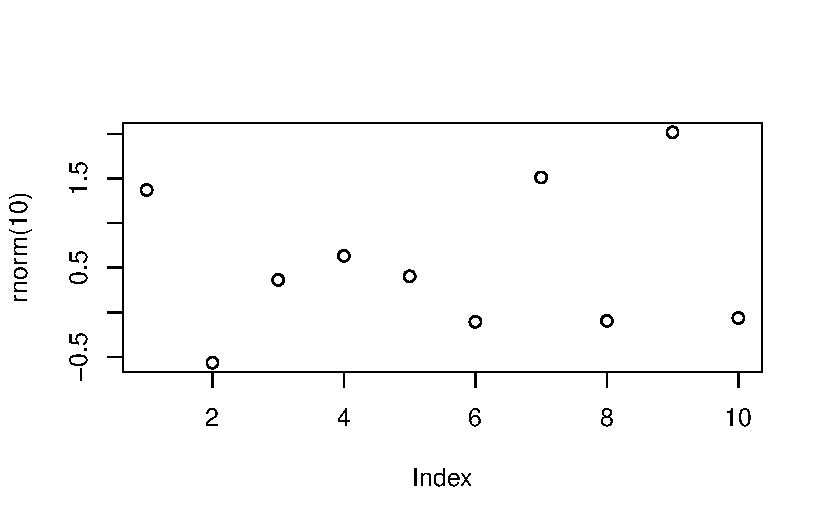
\includegraphics{paper_files/figure-pdf/fig-demo-plot-1.pdf}

}

\caption{\label{fig-demo-plot}A plot of random numbers}

\end{figure}

Figure Figure~\ref{fig-demo-plot} shows how we can have a caption and
cross-reference for a plot. Note that figure label and cross-references
must both be prefixed with \texttt{fig-}

Here is an example of inline code 3.14 in the middle of a sentence.

\hypertarget{discussion}{%
\section{Discussion}\label{discussion}}

\hypertarget{conclusion}{%
\section{Conclusion}\label{conclusion}}

\hypertarget{acknowledgements}{%
\section{Acknowledgements}\label{acknowledgements}}

\newpage

\hypertarget{references}{%
\section{References}\label{references}}

\hypertarget{refs}{}
\begin{CSLReferences}{0}{0}
\end{CSLReferences}

\newpage

\hypertarget{colophon}{%
\subsubsection{Colophon}\label{colophon}}

This report was generated on 2022-12-19 20:02:26 using the following
computational environment and dependencies:

\begin{verbatim}
#> - Session info ---------------------------------------------------------------
#>  setting  value
#>  version  R version 4.2.2 Patched (2022-12-14 r83470)
#>  os       macOS Big Sur ... 10.16
#>  system   x86_64, darwin17.0
#>  ui       X11
#>  language (EN)
#>  collate  en_US.UTF-8
#>  ctype    en_US.UTF-8
#>  tz       America/Los_Angeles
#>  date     2022-12-19
#>  pandoc   2.19.2 @ /usr/local/bin/ (via rmarkdown)
#> 
#> - Packages -------------------------------------------------------------------
#>  package      * version       date (UTC) lib source
#>  askpass        1.1           2019-01-13 [1] CRAN (R 4.2.0)
#>  bayestestR     0.13.0        2022-09-18 [1] CRAN (R 4.2.0)
#>  cachem         1.0.6.9000    2022-06-03 [1] https://r~
#>  callr          3.7.3.9000    2022-11-03 [1] https://r-lib.r-universe.dev (R 4.2.2)
#>  cli            3.4.1.9000    2022-11-09 [1] https://r-lib.r-universe.dev (R 4.2.2)
#>  coda           0.19-4        2020-09-30 [1] CRAN (R 4.2.0)
#>  codetools      0.2-18        2020-11-04 [2] CRAN (R 4.2.2)
#>  crayon         1.5.2         2022-09-29 [1] CRAN (R 4.2.0)
#>  credentials    2.0.0         2022-09-22 [1] https://ropensci.r-universe.dev (R 4.2.1)
#>  datawizard     0.6.5         2022-12-14 [1] CRAN (R 4.2.0)
#>  devtools       2.4.5.9000    2022-10-11 [1] https://r-lib.r-universe.dev (R 4.2.1)
#>  digest         0.6.31        2022-12-11 [1] CRAN (R 4.2.0)
#>  effectsize     0.8.2         2022-10-31 [1] CRAN (R 4.2.1)
#>  ellipsis       0.3.2.9000    2022-06-23 [1] https://r-lib.r-universe.dev (R 4.2.0)
#>  emmeans        1.8.3         2022-12-06 [1] CRAN (R 4.2.2)
#>  estimability   1.4.1         2022-08-05 [1] CRAN (R 4.2.1)
#>  evaluate       0.19.1        2022-12-14 [1] https://r-lib.r-universe.dev (R 4.2.2)
#>  fastmap        1.1.0.9000    2022-05-15 [1] https://r~
#>  fs             1.5.2.9000    2022-05-26 [1] https://r-lib.r-universe.dev (R 4.2.0)
#>  glue           1.6.2.9000    2022-12-20 [1] https://tidyverse.r-universe.dev (R 4.2.2)
#>  htmltools      0.5.4.9000    2022-12-07 [1] https://rstudio.r-universe.dev (R 4.2.2)
#>  htmlwidgets    1.6.0         2022-12-15 [1] CRAN (R 4.2.0)
#>  httpuv         1.6.7.9000    2022-12-15 [1] https://rstudio.r-universe.dev (R 4.2.2)
#>  insight        0.18.8        2022-11-24 [1] CRAN (R 4.2.0)
#>  jsonlite       1.8.4         2022-12-06 [1] CRAN (R 4.2.0)
#>  knitr          1.41.2        2022-12-13 [1] https://yihui.r-universe.dev (R 4.2.2)
#>  later          1.3.0.9000    2022-05-15 [1] https://r~
#>  lattice        0.20-45       2021-09-22 [2] CRAN (R 4.2.2)
#>  lifecycle      1.0.3.9000    2022-10-07 [1] https://r-lib.r-universe.dev (R 4.2.1)
#>  magrittr       2.0.3.9000    2022-05-29 [1] https://tidyverse.r-universe.dev (R 4.2.0)
#>  MASS           7.3-58.1      2022-08-03 [2] CRAN (R 4.2.2)
#>  Matrix         1.5-4         2022-12-17 [2] https://r-forge.r-universe.dev (R 4.2.2)
#>  memoise        2.0.1.9000    2022-05-28 [1] https://r~
#>  mime           0.12.1        2022-06-25 [1] https://yihui.r-universe.dev (R 4.2.1)
#>  miniUI         0.1.1.1       2018-05-18 [1] CRAN (R 4.2.0)
#>  multcomp       1.4-21        2022-11-08 [1] https://r-forge.r-universe.dev (R 4.2.2)
#>  mvtnorm        1.1-3         2021-10-08 [1] CRAN (R 4.2.0)
#>  openssl        2.0.5         2022-12-06 [1] CRAN (R 4.2.0)
#>  papaja       * 0.1.1         2022-07-05 [1] CRAN (R 4.2.0)
#>  parameters     0.20.0        2022-11-21 [1] CRAN (R 4.2.2)
#>  pkgbuild       1.4.0.9000    2022-11-27 [1] https://r-lib.r-universe.dev (R 4.2.2)
#>  pkgload        1.3.2.9000    2022-11-16 [1] https://r-lib.r-universe.dev (R 4.2.2)
#>  prettyunits    1.1.1.9000    2022-05-10 [1] https://r~
#>  processx       3.8.0.9000    2022-10-26 [1] https://r-lib.r-universe.dev (R 4.2.1)
#>  profvis        0.3.7.9000    2022-04-27 [1] https://rstudio.r-universe.dev (R 4.2.0)
#>  promises       1.2.0.9000    2022-04-28 [1] https://rstudio.r-universe.dev (R 4.2.0)
#>  ps             1.7.2.9000    2022-10-27 [1] https://r-lib.r-universe.dev (R 4.2.1)
#>  purrr          0.9000.0.9000 2022-09-14 [1] https://tidyverse.r-universe.dev (R 4.2.1)
#>  R6             2.5.1.9000    2022-11-27 [1] https://r-lib.r-universe.dev (R 4.2.2)
#>  Rcpp           1.0.9         2022-07-08 [1] CRAN (R 4.2.0)
#>  remotes        2.4.2         2021-11-30 [1] CRAN (R 4.2.0)
#>  rlang          1.0.6.9000    2022-10-05 [1] https://r-lib.r-universe.dev (R 4.2.1)
#>  rmarkdown      2.19.1        2022-12-18 [1] Github (rstudio/rmarkdown@c5cf103)
#>  sandwich       3.1-0         2022-08-17 [1] https://r-forge.r-universe.dev (R 4.2.1)
#>  sessioninfo    1.2.2.9000    2022-05-14 [1] https://r~
#>  shiny          1.7.4.9000    2022-12-16 [1] https://rstudio.r-universe.dev (R 4.2.2)
#>  stringi        1.7.8         2022-07-11 [1] CRAN (R 4.2.0)
#>  stringr        1.5.0.9000    2022-12-07 [1] https://tidyverse.r-universe.dev (R 4.2.2)
#>  survival       3.4-0         2022-08-09 [2] CRAN (R 4.2.2)
#>  sys            3.4.1         2022-10-18 [1] CRAN (R 4.2.0)
#>  TH.data        1.1-1         2022-04-26 [1] CRAN (R 4.2.0)
#>  tinylabels   * 0.2.3         2022-02-06 [1] CRAN (R 4.2.0)
#>  urlchecker     1.0.1.9000    2022-05-14 [1] https://r~
#>  usethis        2.1.6.9000    2022-12-13 [1] Github (r-lib/usethis@a98a0e6)
#>  vctrs          0.5.1.9000    2022-12-18 [1] Github (r-lib/vctrs@2d7de76)
#>  xfun           0.35.1        2022-11-16 [1] https://yihui.r-universe.dev (R 4.2.2)
#>  xtable         1.8-6         2022-04-14 [1] https://r-forge.r-universe.dev (R 4.2.0)
#>  yaml           2.3.6         2022-10-18 [1] CRAN (R 4.2.0)
#>  zoo            1.8-12        2022-12-06 [1] https://r-forge.r-universe.dev (R 4.2.2)
#> 
#>  [1] /Users/joey/.Rlibrary
#>  [2] /Library/Frameworks/R.framework/Versions/4.2/Resources/library
#> 
#> ------------------------------------------------------------------------------
\end{verbatim}

The current Git commit details are:

\begin{verbatim}
#> Local:    main /Users/joey/srt
#> Remote:   main @ origin (https://github.com/brainworkup/srt.git)
#> Head:     [c2ad954] 2022-12-20: added PAK pack.lock file
\end{verbatim}


  \bibliography{references.bib}


\end{document}
